\subsection{Construction}
\begin{frame}{Social Network}
This social network is of a particular kind called \emph{two-mode networks} which consists of a set of actors (seiyuu) and events (anime).
\vspace{15pt}

Details to consider:
\begin{itemize}
\item We can choose between anime and seiyuu as nodes.
\item Nodes are time dependant (since they have debut year).
\item Edge or relationship definition:
	\begin{itemize}
	\item How many works in common?
	\item Which time frame?
	\end{itemize}
\end{itemize}
\vspace{15pt}
\end{frame}
%-------------------------------------------------------------------------

\begin{frame}
We compared two graph definitions using \emph{seiyuu as nodes} and, as edge definition:
\begin{itemize}
\item at least 1 work in common
\item at least 10 works in common
\end{itemize}
Both of them during the time frame between the first debut registered (1960) and the year of observation.
\end{frame}
%-------------------------------------------------------------------------

\subsection{Analysis}
\begin{frame}{One work in common}
\begin{figure}
	\begin{subfigure}{.6\linewidth}
		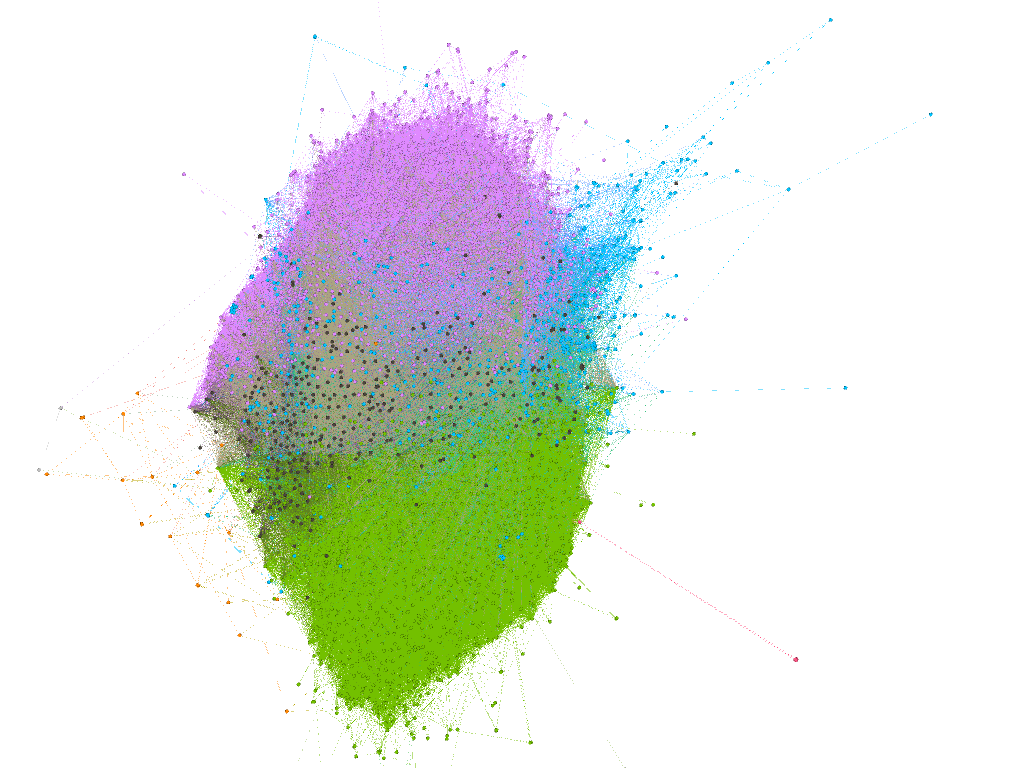
\includegraphics[scale=0.27, left]{graphics/atLeast1WorkCommunity.png} 
	\end{subfigure}%
	\begin{subfigure}{.4\linewidth}
		\begin{description}
		\item[Avg degree] 267
		\item[Graph density] 0.09
		\item[Modularity] 0.2
		\item[Network diameter] 6
		\item[Connected components] 18
		\end{description}
	\end{subfigure}
\end{figure}
\end{frame}
%-------------------------------------------------------------------------

\begin{frame}{Ten works in common}
\begin{figure}
	\begin{subfigure}{.55\linewidth}
		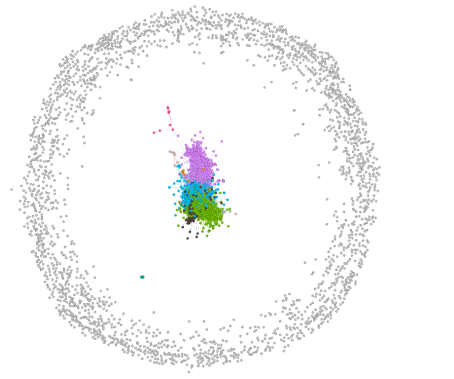
\includegraphics[scale=0.55, left]{graphics/atLeast10WorksCommunity.png} 
	\end{subfigure}%
	\begin{subfigure}{.45\linewidth}
		\begin{description}
		\item[Avg degree] 9
		\item[Graph density] 0.003
		\item[Modularity] 0.29
		\item[Network diameter] 7
		\item[Connected components] 2261
		\end{description}
	\end{subfigure}
\end{figure}
\end{frame}
%-------------------------------------------------------------------------

\begin{frame}{Features}
\begin{description}
	\item [Strongly connected] With merely $\sim$3000 nodes it has $\sim$400000 edges when only one work in common is required and $\sim$14000 edges when asking for 10 or more. 
	\item [Big cluster] Thightly interconnected and big cluster surrounded by poorly or not connected nodes. (99\% of the nodes of one work in common graph and 23\% of 10 works in common). 
	\item [Communities] We can see at least four clear communities in each graph.
	\item [Nodes] This graph is accumulative, so long carrier almost always means a strong node.
\end{description}
\end{frame}
%-------------------------------------------------------------------------

\begin{frame}{Edge growth}
\begin{figure}
	\centering
	\begin{subfigure}{.5\columnwidth}
		\centering
		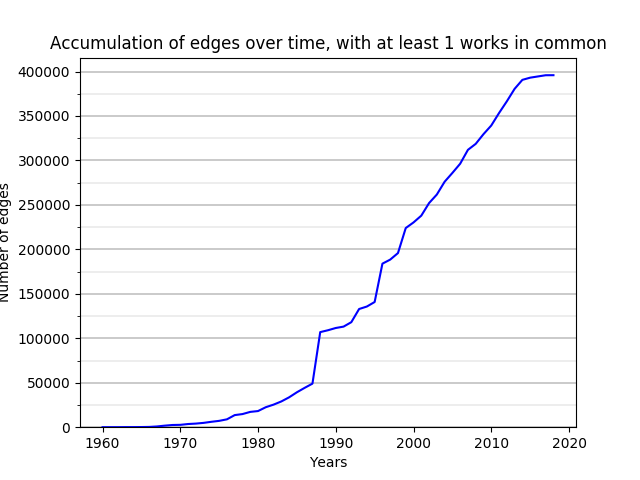
\includegraphics[scale=0.35]{graphics/accumulationEdges_1_1960-2018.png}
	\end{subfigure}%
	\begin{subfigure}{.5\columnwidth}
		\centering
		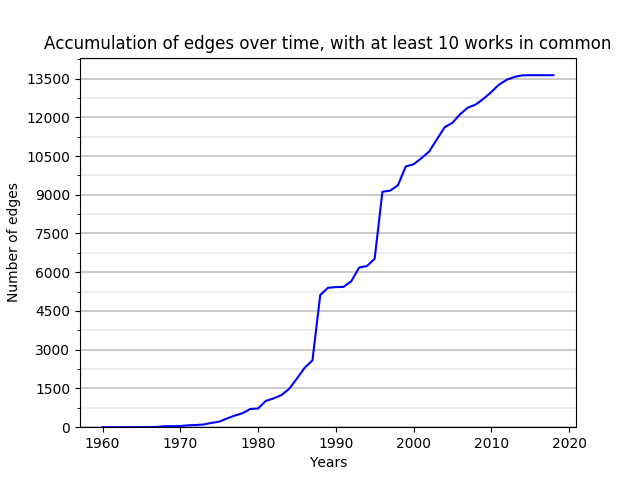
\includegraphics[scale=0.35]{graphics/accumulationEdges_10_1960-2018.png}
	\end{subfigure}
\end{figure}
\begin{itemize}
\item Edge growth follows the same distribution with 1 and 10 works in common
\end{itemize}
\end{frame}
%-------------------------------------------------------------------------

\begin{frame}{Node growth}
\begin{center}
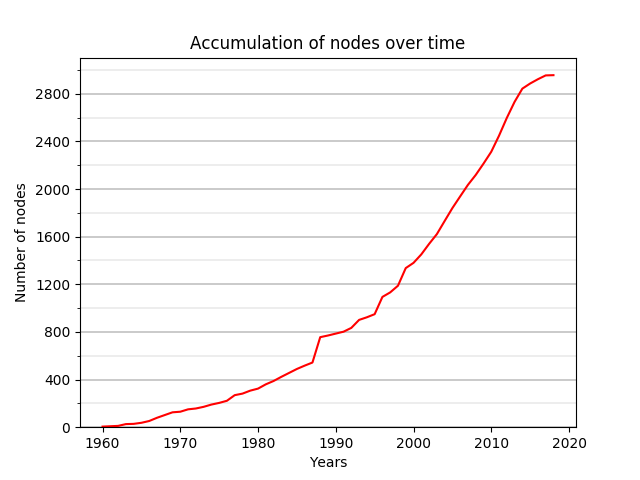
\includegraphics[scale=0.5]{graphics/nodesAccumulation.png} 
\end{center}
\begin{itemize}
\item More than half of the nodes are from last 18 years (2000 to 2018)
\end{itemize}
\end{frame}
%-------------------------------------------------------------------------

\begin{frame}{Top 5 degree}
\begin{table}[!htb]
    \begin{minipage}{.5\textwidth}
        \centering
            \begin{tabular}{|l|c|}
				\hline
				Name & Degree \\ 
				\hline
				Takehito Koyasu & 1545 \\ 
				\hline
				Akira Ishida & 1488 \\ 
				\hline
				Mamiko Noto & 1422 \\ 
				\hline
				Nobuo Tobita & 1417 \\ 
				\hline
				Daisuke Namikawa & 1390 \\ 
				\hline
			\end{tabular}
            \caption{One work in common}
    \end{minipage}%
    \begin{minipage}{.6\textwidth}
        \centering
        \begin{tabular}{|l|c|}
				\hline
				Name & Degree \\
				\hline
				Takehito Koyasu & 311 \\
				\hline
				Akira Ishida & 273 \\
				\hline
				Mamiko Noto & 258 \\
				\hline
				Daisuke Namikawa & 232 \\
				\hline
				Katsuyuki Konishi & 229 \\
				\hline
			\end{tabular}
            \caption{Ten works in common}
    \end{minipage}
\end{table}
\end{frame}
%-------------------------------------------------------------------------

\begin{frame}{Top 5 betweenness centrality}
\begin{table}[!htb]
    \begin{minipage}{.5\textwidth}
        \centering
            \begin{tabular}{|l|c|}
				\hline
				Name & BtwC \\
				\hline
				Takehito Koyasu & 49982.52 \\
				\hline
				Akira Ishida & 40221.50 \\
				\hline
				Daisuke Namikawa & 30448.43 \\
				\hline
				Nobuo Tobita & 29363.25 \\
				\hline
				Mamiko Noto & 29168.18 \\
				\hline
		\end{tabular}
        \caption{One work in common}
    \end{minipage}%
    \begin{minipage}{.5\textwidth}
        \centering
        \begin{tabular}{|l|c|}
				\hline
				Name & BtwC \\
				\hline
				Takehito Koyasu & 18489.44 \\
				\hline
				Mamiko Noto & 10988.96 \\
				\hline
				Daisuke Namikawa & 9570.48 \\
				\hline
				Akira Ishida & 8299.19 \\
				\hline
				Rie Kugimiya & 7560.16 \\
				\hline
		\end{tabular}
        \caption{Ten works in common}
    \end{minipage}
\end{table}
\end{frame}
%-------------------------------------------------------------------------

\begin{frame}
Both networks have fairly similar top 5s so it points to them having similar structure and connections amoung their nodes, aside from actual values.
\vspace{10pt}

From now on our graph definition will be:
\begin{description}
\item[Node] Seiyuu
\item[Edge] At least 10 works in common from 1960 to year of observation.
\end{description}
\vspace{10pt}

Because requiring more jobs in common means less amount of edges, this leaves a more understandable graph and we verified it does without changing its structure so much.
\end{frame}